\section{Captions, labels and references}

Images can be captioned, labelled and referenced by means of the figure environment, as shown below:

\begin{tcolorbox}
\begin{verbatim}
    \documentclass{article}
    \usepackage{graphicx}
    \graphicspath{{images/}}
 
    \begin{document}

    \begin{figure}[h]
        \centering
        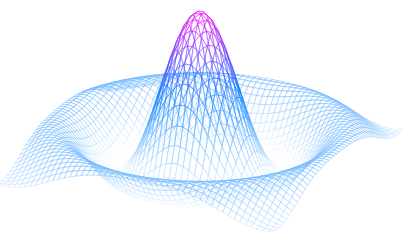
\includegraphics[width=0.75\textwidth]{mesh}
        \caption{A nice plot.}
        \label{fig:mesh1}
    \end{figure}
 
    As you can see in figure \ref{fig:mesh1}, the function grows 
    near the origin. This example is on page \pageref{fig:mesh1}.

    \end{document}
\end{verbatim}
\end{tcolorbox}

This example produces the following output:

\begin{figure}[h]
\begin{mdframed}
    \begin{Center}
        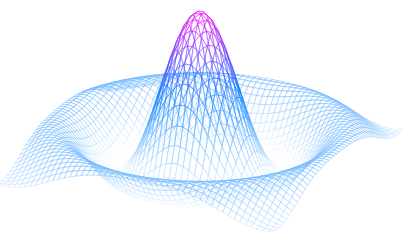
\includegraphics[width=0.25\textwidth]{mesh}
        \caption{a nice plot}
        \label{fig:mesh1}
    \end{Center}

    \-\hspace{20pt}As you can see in figure \ref{fig:mesh1}, the function grows near the origin. This example is on page \pageref{fig:mesh1}.
\end{mdframed}
\end{figure}

There are several noteworthy commands in the example:

\begin{itemize}
    \item \verb|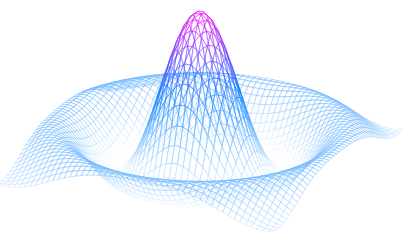
\includegraphics[width=0.75\textwidth]{mesh}|: This form of \\\verb|\includegraphics| instructs \LaTeX\ to set the figure’s width to 75\verb|%| of the text width—whose value is stored in the \verb|\textwidth| command.
    \item \verb|\caption{A nice plot.}|: As its name suggests, this command sets the figure caption which can be placed above or below the figure. If you create a list of figures this caption will be used in that list.
    \item \verb|\label{fig:mesh1}|: To reference this image within your document you give it a label using the \verb|\label| command. The label is used to generate a number for the image and, combined with the next command, will allow you to reference it.
    \item \verb|\ref{fig:mesh1}|: This code will be substituted by the number corresponding to the referenced figure.
\end{itemize}

Images incorporated in a \LaTeX\ document should be placed inside a figure environment, or similar, so that \LaTeX\ can automatically position the image at a suitable location in your document.

Further guidance is contained in the following Overleaf help articles:

\begin{itemize}
    \item \href{https://www.overleaf.com/learn/latex/Positioning_of_Figures}{Positioning of Figures}
    \item \href{https://www.overleaf.com/learn/latex/Inserting_Images}{Inserting Images}
\end{itemize}